\section{SENSITIVITY ANALYSIS AND EXPERIMENTATION}
The proposed sensitivity analysis consists of varying the radius $d$ 10\% below and above its original value. In this case, we extracted the average number of diabetic agents in the last 300 ticks (steady-state) and it was plotted against the current radius in \cref{fig:sens}. It can be observed that the output does not change drastically, therefore the model is not highly sensitive to the radius.
\begin{figure}[H]
    \centering
    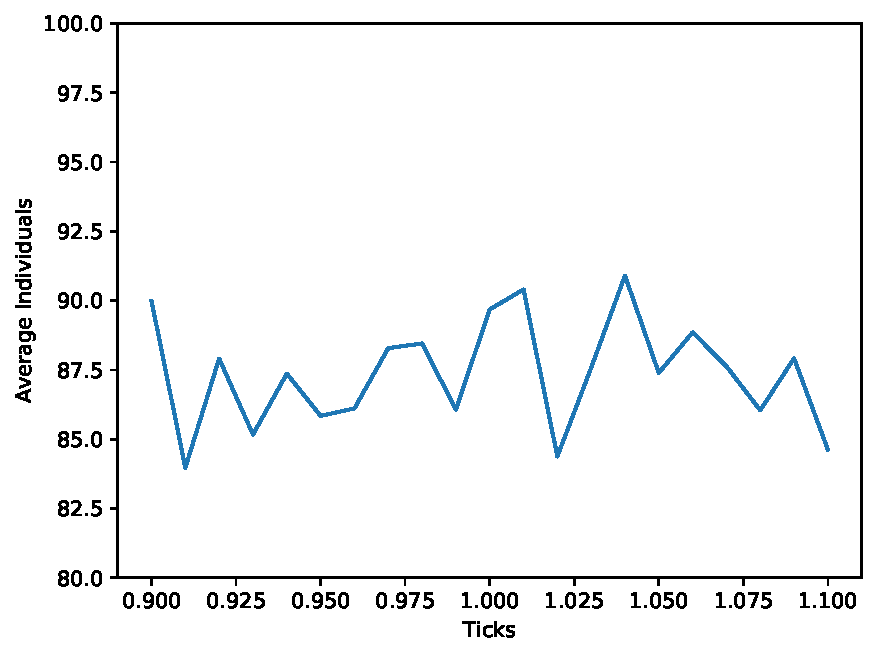
\includegraphics[width=0.3\columnwidth]{files/sensitivity-diabetes.pdf}
    \caption{Sensitivity analysis.}
    \label{fig:sens}
\end{figure}
